

\subsection{Vector Arithmetic}
\label{subsec:vector-arithmetic}

This section explains basic arithmetic of vector and matrix computations, and advanced concepts such as vector/plane projection and basis of planes (or spaces). 


\begin{tcolorbox}[title={\textbf{\tboxdef{\ref*{subsec:vector-arithmetic}} Vector Arithmetic}}]

\begin{itemize}
\item \textbf{Addition:} Given two $n \times 1$ vectors (i.e., $n$-dimensional vectors) composed of $n$ numbers each:

$\vec{a} = (a_0, a_1, \gap{$\cdots$}, a_{n-1})$, $\vec{b} = (b_0, b_1, \gap{$\cdots$}, b_{n-1})$

$ $

Vector addition is defined as: 

$ \vec{a} + \vec{b} = (a_0 + b_0, \text{ } a_1  +  b_1, \text{ } \gap{$\cdots$}, \text{ } a_{n-1}  +  b_{n-1})$

$ $

\item \textbf{Dot Product:} Given two $n$-dimensional vectors:

$\vec{a} = (a_0, a_1, \gap{$\cdots$}, a_{n-1})$, $\vec{b} = (b_0, b_1, \gap{$\cdots$}, b_{n-1})$

$ $

Dot product is defined as: 

$\langle \vec{a}, \vec{b} \rangle =  \vec{a} \cdot \vec{b} = a_0 b_0 + a_1 b_1 + \gap{$\cdots$}, + a_{n-1} b_{n-1}$.

More formally, $\vec{a} \cdot \vec{b} = |a||b|\cos\theta$, where $\theta$ is the angle between the two vectors. As $\vec{a}$ and $\vec{b}$ point at the same direction, $\vec{a} \cdot \vec{b}$ convergest to a maximized value. As $\vec{a}$ and $\vec{b}$ have an orthogonal direction, $\vec{a} \cdot \vec{b}$ converges to  0. 

$ $


\item \textbf{Hadamard Product:} Given two $n$-dimensional vectors:

$\vec{a} = (a_0, a_1, \gap{$\cdots$}, a_{n-1})$, $\vec{b} = (b_0, b_1, \gap{$\cdots$}, b_{n-1})$

$ $

Hadamard product is defined as: 

$\vec{a} \odot \vec{b} = (a_0 b_0, \text{ } a_1 b_1, \text{ } \gap{$\cdots$}, \text{ } a_{n-1} b_{n-1})$

$ $

\item \textbf{Hermitian Product:} Given two $n$-dimensional complex vectors:

$\vec{a} = (a_0 + i \cdot a'_0, \text{ } a_1+ i\cdot a'_1, \text{ } \gap{$\cdots$},\text{ }  a_{n-1}+ i\cdot a'_{n-1})$ 

$\vec{b} = (b_0 + i\cdot b'_0, \text{ } b_1 + i\cdot b'_1, \text{ } \gap{$\cdots$}, \text{ } b_{n-1} + i\cdot b'_{n-1})$

$ $

Hermitian product is a dot product with the 2nd operand as a conjugate (\autoref{subsec:imaginary}): 

$\langle\langle \vec{a}, \vec{b} \rangle\rangle =  \vec{a} \cdot \overline{\vec{b}} $

$ = (a_0 + i \cdot a'_0, \text{ } a_1+ i\cdot a'_1, \text{ } \gap{$\cdots$},\text{ } a_{n-1}+ i\cdot a'_{n-1})  \cdot (b_0 - i\cdot b'_0, \text{ } b_1 - i\cdot b'_1, \text{ } \gap{$\cdots$}, \text{ } b_{n-1} - i\cdot b'_{n-1})$




\end{itemize}
\end{tcolorbox}




\subsection{Various Types of Matrix}
\label{subsec:vandermonde}


\begin{tcolorbox}[title={\textbf{\tboxdef{\ref*{subsec:vandermonde}} Matrices}}]


\begin{itemize}

\item An $n \times n$ \textbf{identity matrix} and a \textbf{reverse identity matrix} are defined as:

$I_n = \begin{bmatrix}
1 & 0 & 0 & \cdots & 0\\
0 & 1 & 0 & \cdots & 0 \\
0 & 0 & 1 & \cdots & 0 \\
\vdots & \vdots & \vdots & \ddots & \vdots \\
0 & 0 & 0 & \cdots & 1 \\
\end{bmatrix}$, $I^R_n = \begin{bmatrix}
0 & \cdots & 0 & 0 & 1\\
0 & \cdots & 0 & 1 & 0 \\
0 & \cdots & 1 & 0 & 0 \\
\vdots & \iddots & \vdots & \vdots & \vdots \\
1 & 0 & 0 & \cdots & 0 \\
\end{bmatrix}$

$ $

\item The \textbf{transpose of a matrix} $X$ is defined as element-wise swapping along the diagonal line, denoted as $X^T$, which is:


$X = \begin{bmatrix}
a_1 & a_2 & a_3 & \cdots & a_n\\
b_1 & b_2 & b_3 & \cdots & b_n \\
c_1 & c_2 & c_3 & \cdots & c_n \\
\vdots & \vdots & \vdots & \ddots & \vdots \\
m_1 & m_2 & m_3 & \cdots & m_n \\
\end{bmatrix}$, $X^T = \begin{bmatrix}
a_1 & b_1 & c_1 & \cdots & m_1\\
a_2 & b_2 & c_2 & \cdots & m_2\\
a_3 & b_3 & c_3 & \cdots & m_3\\
\vdots & \vdots & \vdots & \ddots & \vdots \\
a_n & b_n & c_n & \cdots & m_n\\
\end{bmatrix}$

$ $


\item A \textbf{Vandermonde matrix} is an $(m + 1) \times (n + 1)$ matrix defined as:

$V(x_0, x_1, \cdots, x_{m}) = \begin{bmatrix}
1 & x_0 & x_0^2 & \cdots & x_0^n\\
1 & x_1 & x_1^2 & \cdots & x_1^n \\
1 & x_2 & x_2^2 & \cdots & x_2^n \\
\vdots & \vdots & \vdots & \ddots & \vdots \\
1 & x_m & x_m^2 & \cdots & x_m^{n} \\
\end{bmatrix}$

%A Vandermonde matrix is often used for representing $m$ different $n$-degree polynomials.

\end{itemize}

\end{tcolorbox}


 





\subsection{Matrix Arithmetic}
\label{subsec:matrix-arithmetic}


Matrix-to-vector multiplication and matrix-to-matrix multiplication are defined as follows:




\begin{tcolorbox}[title={\textbf{\tboxdef{\ref*{subsec:matrix-arithmetic}} Matrix Arithmetic}}]

\begin{itemize}
\item \textbf{Matrix-to-Vector Multipication:} Given a $m \times n$ matrix $A$ and a $n$-dimensional vector $x$: 


$A = \begin{bmatrix}
 a_{\langle 1, 1\rangle} & a_{\langle 1, 2\rangle} & a_{\langle 1, 3\rangle} & \cdots & a_{\langle 1, n\rangle}\\
 a_{\langle 2, 1\rangle} & a_{\langle 2, 2\rangle} & a_{\langle 2, 3\rangle} & \cdots & a_{\langle 2, n\rangle} \\
 a_{\langle 3, 1\rangle} & a_{\langle 3, 2\rangle} & a_{\langle 3, 3\rangle} & \cdots & a_{\langle 3, n\rangle} \\
\vdots & \vdots & \vdots & \ddots & \vdots \\
 a_{\langle m, 1\rangle} & a_{\langle m, 2\rangle} & a_{\langle m, 3\rangle} & \cdots & a_{\langle m, n\rangle} \\
\end{bmatrix} = \begin{bmatrix} 
\vec{a}_{\langle 1, * \rangle} \\ 
\vec{a}_{\langle 2, * \rangle} \\ 
\vec{a}_{\langle 3, * \rangle} \\ 
\vdots\\
\vec{a}_{\langle m, * \rangle} \\ 
\end{bmatrix}, \text{ } \vec{x} = (x_1, x_2, \cdots, x_{n})$


$ $

The result of $A \cdot \vec{x}$ is an $n$-dimensional vector computed as:

$A \cdot \vec{x} = \Big(\vec{a}_{\langle 1, * \rangle} \cdot \vec{x}, \text{ } \vec{a}_{\langle 2, * \rangle} \cdot \vec{x}, \text{ }\cdots,\text{ } \vec{a}_{\langle m, * \rangle} \cdot \vec{x} \Big) = \left(\sum\limits_{i=1}^{n} a_{1, i} \cdot  x_i, \text{ } \sum\limits_{i=1}^{n}  a_{2, i} \cdot x_i, \gap{$\cdots$}, \text{ } \sum\limits_{i=1}^{n} a_{m, i} \cdot x_i \right)$


$ $


\item \textbf{Matrix-to-Matrix Multiplication:} Given a $m \times n$ matrix $A$ and a $n \times k$ matrix $B$: 



$A = \begin{bmatrix}
 a_{\langle 1, 1\rangle} & a_{\langle 1, 2\rangle} & a_{\langle 1, 3\rangle} & \cdots & a_{\langle 1, n\rangle}\\
 a_{\langle 2, 1\rangle} & a_{\langle 2, 2\rangle} & a_{\langle 2, 3\rangle} & \cdots & a_{\langle 2, n\rangle} \\
 a_{\langle 3, 1\rangle} & a_{\langle 3, 2\rangle} & a_{\langle 3, 3\rangle} & \cdots & a_{\langle 3, n\rangle} \\
\vdots & \vdots & \vdots & \ddots & \vdots \\
 a_{\langle m, 1\rangle} & a_{\langle m, 2\rangle} & a_{\langle m, 3\rangle} & \cdots & a_{\langle m, n\rangle} \\
\end{bmatrix}$, $B = \begin{bmatrix}
 b_{\langle 1, 1\rangle} & b_{\langle 1, 2\rangle} & b_{\langle 1, 3\rangle} & \cdots & b_{\langle 1, k\rangle}\\
 b_{\langle 2, 1\rangle} & b_{\langle 2, 2\rangle} & b_{\langle 2, 3\rangle} & \cdots & b_{\langle 2, k\rangle} \\
 b_{\langle 3, 1\rangle} & b_{\langle 3, 2\rangle} & b_{\langle 3, 3\rangle} & \cdots & b_{\langle 3, k\rangle} \\
\vdots & \vdots & \vdots & \ddots & \vdots \\
 b_{\langle n, 1\rangle} & b_{\langle n, 2\rangle} & b_{\langle n, 3\rangle} & \cdots & b_{\langle n, k\rangle} \\
\end{bmatrix}$

$ $

The result of $A \cdot B$ is a $m \times k$ matrix computed as:

$A \cdot B = \begin{bmatrix}
\sum\limits_{i=1}^{n}a_{\langle 1, i\rangle}b_{\langle i, 1\rangle} & \sum\limits_{i=1}^{n}a_{\langle 1, i\rangle}b_{\langle i, 2\rangle} & \sum\limits_{i=1}^{n}a_{\langle 1, i\rangle}b_{\langle i, 3\rangle} & \cdots & \sum\limits_{i=1}^{n}a_{\langle 1, i\rangle}b_{\langle i, k\rangle} \\
\sum\limits_{i=1}^{n}a_{\langle 2, i\rangle}b_{\langle i, 1\rangle} & \sum\limits_{i=1}^{n}a_{\langle 2, i\rangle}b_{\langle i, 2\rangle} & \sum\limits_{i=1}^{n}a_{\langle 2, i\rangle}b_{\langle i, 3\rangle} & \cdots & \sum\limits_{i=1}^{n}a_{\langle 2, i\rangle}b_{\langle i, k\rangle} \\
\sum\limits_{i=1}^{n}a_{\langle 3, i\rangle}b_{\langle i, 1\rangle} & \sum\limits_{i=1}^{n}a_{\langle 3, i\rangle}b_{\langle i, 2\rangle} & \sum\limits_{i=1}^{n}a_{\langle 3, i\rangle}b_{\langle i, 3\rangle} & \cdots & \sum\limits_{i=1}^{n}a_{\langle 3, i\rangle}b_{\langle i, k\rangle} \\
\vdots & \vdots & \vdots & \ddots & \vdots \\
\sum\limits_{i=1}^{n}a_{\langle m, i\rangle}b_{\langle i, 1\rangle}
& \sum\limits_{i=1}^{n}a_{\langle m, i\rangle}b_{\langle i, 2\rangle} & \sum\limits_{i=1}^{n}a_{\langle m, i\rangle}b_{\langle i, 3\rangle} & \cdots & \sum\limits_{i=1}^{n}a_{\langle m, i\rangle}b_{\langle i, k\rangle} \\
\end{bmatrix}$


\end{itemize}
\end{tcolorbox}

Given the above definitions of matrix and vector arithmetic, the following algebraic properties can be derived:

\begin{tcolorbox}[title={\textbf{\tboxtheorem{\ref*{subsec:matrix-arithmetic}} Matrix Arithmetic Properties}}]

\begin{itemize}

\item \textbf{Associative:} 

$(AB)C = A(BC)$

$A(Bx) = (AB)x$


$ $

 
\item \textbf{Distributive:} 

$A(x + y) = Ax + Ay$

$A(x \odot y) = Ax \odot Ay $

$A\langle x, y\rangle = \langle Ax, Ay\rangle$

$A\langle \langle x, y\rangle\rangle = \langle\langle Ax, Ay\rangle\rangle$

(However, $Ax \cdot Ay \neq A(x \cdot y)$, because the resulting dimensions do not match. Also, $A(x \odot y) \neq Ax \odot Ay $)

$ $

\item \textbf{NOT Commutative:} 

$Ax \neq xA$

$AB \neq BA$


\end{itemize}
\end{tcolorbox}

\begin{proof}

$ $

The properties described in \ref*{subsec:matrix-arithmetic} can be demonstrated by expanding the formulas of both sides each equation by using a variable representation for each element in the vectors/matrices and comparing the resulting formulas. We leave this expansion as an exercise for the reader.

\end{proof}


\subsection{Projection}
\label{subsec:projection}

There are two types of projections: a vector projection and an orthogonal (i.e., plane) projection. 



\begin{figure}[!h]
    \centering
    \subfloat[Vector Projection \href{https://upload.wikimedia.org/wikipedia/commons/thumb/9/98/Projection_and_rejection.png/200px-Projection_and_rejection.png}{(Source)}]{
  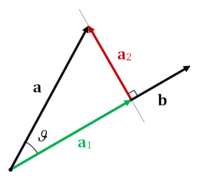
\includegraphics[width=0.25\linewidth]{figures/vector-projection.png}

  \label{fig:vector-projection}
}
    \subfloat[Orthogonal (Plane/Subspace) Projection \href{https://www.researchgate.net/publication/333616378/figure/fig2/AS:766235117617152@1559696096437/Geometric-illustration-of-the-orthogonal-projection-operator-P-A-vector-x-R-m-is.png}{(Source)}]{
  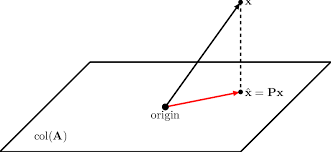
\includegraphics[width=0.4\linewidth]{figures/orthogonal-projection.png}

  \label{fig:orthogonal-projection}
}
  \caption{}
\end{figure}


\para{Vector Projection:} Given two vectors $\vec{a}$ and $\vec{b}$ in the same $n$-dimensional vector space, the vector projection $\textsf{Proj}_{\vec{b}}(\vec{a})$ measures how much $\vec{a}$ contains the element of $\vec{b}$ (i.e., filtering $\vec{a}$ by $\vec{b}$). In the example of \autoref{fig:vector-projection}, $\vec{a}$'s projection on $\vec{b}$ is $\vec{a}_1$, where the length of $\vec{a}_1$ is geometrically $||a_1|| = ||a|| \cos \theta = ||a||\dfrac{a \cdot b}{||a||\cdot||b||} = \dfrac{a \cdot b}{||b||}$. Let $\vec{b'}$ be a unit vector of $\vec{b}$, that is $\vec{b'} = \dfrac{\vec{b}}{||b||}$. Then, $\vec{a}_1 = ||a_1||\cdot\vec{b'} = \dfrac{a \cdot b}{||b||} \cdot \dfrac{\vec{b}}{||b||} = \dfrac{a \cdot b}{||b||^2}\vec{b}$. Thus, $\textsf{Proj}_{\vec{b}}(\vec{a}) = \dfrac{a \cdot b}{||b||^2}\vec{b}$.

\para{Orthogonal Projection:} Given the vector $\vec{x}$ and a set of mutually orthogonal vectors $\vec{p}_0, \vec{p}_1, \cdots, \vec{p}_{n-1}$ which span the plane (or subspace) $P$, the orthogonal projection $\textsf{Proj}_P(\vec{x})$ measures how much element of plane $P$ is contained in $\vec{x}$ (i.e., filtering $\vec{x}$ by plane $P$). In the example of \autoref{fig:orthogonal-projection}, vector $\vec{x}$'s projection on plane $P$ is shown as a red arrow, which is computed by summing the projection of $\vec{x}$ on each of the mutually orthogonal vectors $\vec{p}_0, \vec{p}_1, \cdots, \vec{p}_{n-1}$ that span plane $P$. This is equivalent to $\textsf{Proj}_P(\vec{a}) = \sum\limits_{i=0}^{n-1} \textsf{Proj}_{\vec{p}_i}(\vec{a})$. The computation of $\textsf{Proj}_P(\vec{x})$ can be thought of transforming $\vec{v}$ into a different coordinate system that expresses the vector space in terms of $n$ mutually orthogonal vectors. 

\begin{tcolorbox}[title={\textbf{\tboxdef{\ref*{subsec:projection}} Vector and Orthogonal Projections}}]

\begin{itemize}

\item \textbf{Vector Projection:} Given two vectors $\vec{a}$ and $\vec{b}$ in the same vector space, the vector projection of $\vec{a}$ on $\vec{b}$ is:

$\textsf{Proj}_{\vec{b}}(\vec{a}) = \vec{a}_p = \vec{a} \cos \theta = \dfrac{\vec{a} \cdot \vec{b}}{||b||^2} \vec{b}$

$ $

\item \textbf{Orthogonal Basis:} If the $n$-dimensional plane (or subspace) $P$ is spanned by the mutually orthogonal $n$-dimensional vectors $\vec{p}_0, \vec{p}_1, \cdots, \vec{p}_n$, 

then the matrix $P = \begin{bmatrix} 
\vec{p}_0\\
\vec{p}_1\\
\vdots\\
\vec{p}_{n-1}\\
\end{bmatrix}
$
is defined to be an orthogonal basis of plane $P$. 


\item \textbf{Orthogonal Projection:} Given the orthogonal basis matrix $P = \begin{bmatrix} 
\vec{p}_0\\
\vec{p}_1\\
\vdots\\
\vec{p}_{n-1}\\
\end{bmatrix}
$, 

vector $\vec{a}$'s orthogonal projection on $P$ is:

$\textsf{Proj}_P(\vec{a}) = \sum\limits_{i=1}^n \textsf{Proj}_{\vec{p}_i}(\vec{a})$



\end{itemize}


\end{tcolorbox}


Based on the definition of orthogonal projection, the following properties are derived:  

\para{Orthogonal Basis:} In an $n$-dimensional vector space, any mutually orthogonal $n$ vectors in the vector space span a plane (or subspace) $P$ that is identical to the entire vector space. Further, an orthogonal projection of any vector in the vector space on $P$ is guaranteed to be a unique vector.

\para{Non-orthogonal Basis:} In an $n$-dimensional vector space, suppose some $n$ non-orthogonal vectors satisfy the following two conditions: (i) they span the entire vector space; (ii) they are linearly independent (i.e., one vector cannot be expressed as a linear combination of the other vectors). Then, the $n \times n$ matrix $P$ comprised of these $n$ vectors forms a basis of the entire vector space $V$, and the matrix-to-vector multiplication $P\vec{v}$ for each $\vec{v}$ in the vector space is guaranteed to give a unique vector. However, the formula $\textsf{Proj}_P(\vec{v})$ is not a valid geometric projection of the vector $\vec{\vec{v}}$ on $P$, because the $n$ basis vectors are non-orthogonal. Yet, the computation of $P\vec{v}$ can be thought of as uniquely transforming $\vec{v}$ into a different coordinate system that expresses the vector space in respect to $n$ non-orthogonal vectors in $P$. 

\begin{tcolorbox}[title={\textbf{\tboxtheorem{\ref*{subsec:projection}} Uniqueness of Transformed Vectors}}]

\begin{itemize}
\item  \textbf{Orthogonal Basis:} If some $n$ vectors are a orthogonal basis of the plane $P$ in the $n$-dimensional vector space, then $P$ is the same as the entire vector space, and $\textsf{Proj}_P(v)$ for every vector $\vec{v}$ in the vector space is guaranteed to be a unique vector.
\item \textbf{Non-orthogonal Basis:} If some $n$ vectors are a non-orthogonal basis of the plane $P$ in the $n$-dimensional vector space (i.e., each vector is linearly independent and they span $P$), then $P$ is the same as the entire vector space, and $P\vec{v}$ is guaranteed to result in a unique vector.  
\end{itemize}
\end{tcolorbox}




\subsection{Basis of a Polynomial Ring}
\label{subsec:polynomial-ring-basis}

Given an $(n-1)$-degree polynomial ring $\mathbb{Z}[X] / (X^n + 1)$, a basis of the polynomial ring is defined to be a set of polynomials that satisfy the following two requirements:

\begin{itemize}

\item \textbf{Linear Independence}: Each polynomial in the basis set cannot be expressed as a linear combination of the other polynomials in the same set
\item \textbf{Spanning the Polynomial Ring:} A linear combinations of the polynomials in the basis set can express any polynomials in the polynomial ring
\end{itemize}

Note that for a $(n-1)$-degree polynomial ring, the number of polynomials that form a basis of the polynomial ring is exactly $n$.


\subsection{Isomorphism between Polynomials and Vectors over Integers}
\label{subsec:poly-vector-transformation}



Now, let's define a mapping $\sigma$ from the $(n-1)$-degree polynomial ring to the $n$-dimensional vector space, such that an input polynomial's list of $y$ values evaluated at $n$ distinct $x$ coordinates (e.g., $x_0, x_1, \cdots, x_{n-1}$) form the mapping's output vector. Technically, $\sigma$ is defined as:

$\sigma: f(x) \in \mathbb{Z}[X] / (X^n + 1) \text{ } \longrightarrow \text{ } (f(x_0), f(x_1), f(x_2), \cdots, f(x_{n-1})) \in \mathbb{Z}^n$

Now, we will explain why the mapping $\sigma$ is isomorphic, which means that $\sigma$ is a bijective one-to-one mapping from $\mathbb{Z}[X] / (X^n + 1)$ to $\mathbb{Z}^n$ and the algebraic operations $(+, \cdot)$ of the mapped elements preserve correctness with homomorphism.

$ $

\para{Bijective:} In the $(n-1)$-degree polynomial ring, the a list of $y$ values evaluated at some statically chosen $n$ distinct $x$ coordinates define a unique polynomial, because algebraically there exists only one $(n-1)$-degree (or a lesser degree) polynomial that passes each given set of $n$ distinct $(x, y)$ coordinates. We proved this in Lagrange Polynomial Interpolation (Theorem~\ref*{sec:polynomial-interpolation} in \autoref{sec:polynomial-interpolation}). 

$ $

\para{Homomorphic:} The homomorphism of the mapping $\sigma$ on the $(+, \cdot)$ operations mean that the following two relationships hold: 

$\sigma(f_a(X) + f_b(X)) = \sigma(f_a(X)) + \sigma(f_b(X))$

$\sigma(f_a(X) \cdot f_b(X)) = \sigma(f_a(X)) \odot \sigma(f_b(X))$ \textcolor{red}{ \text{ } \# $\odot$ is Hadamard vector multiplication (Summary~\ref*{subsec:vector-arithmetic})}

$ $

To prove our $\sigma$ mapping's homomorphism, let's denote the input polynomials $f_a(X)$, $f_b(X)$, and their $\sigma$-mapped output vectors as follows:


$f_a(X) = a_0 + a_1X + a_2X^2 + \cdots + a_{n-1}X^{n-1}$

$ \sigma(f_a(X)) = \left({f_a(x_0)}, {f_a(x_1)}, {f_a(x_2)}, \cdots, {f_a(x_{n-1}}) \right)  = \left(\sum\limits_{i=0}^{n-1}a_i(x_0)^i, \sum\limits_{i=0}^{n-1}a_i(x_1)^i, \sum\limits_{i=0}^{n-1}a_i(x_2)^i, \cdots, \sum\limits_{i=0}^{n-1}a_i(x_{n-1})^i\right)$


$ $

$f_b(X) = b_0 + b_1X + b_2X^2 + \cdots + b_{n-1}X^{n-1}$

$ \sigma(f_b(X)) = \left({f_b(x_0)}, {f_b(x_1)}, {f_b(x_2)}, \cdots, {f_b(x_{n-1}}) \right) = \left(\sum\limits_{i=0}^{n-1}b_i(x_0)^i, \sum\limits_{i=0}^{n-1}b_i(x_1)^i, \sum\limits_{i=0}^{n-1}b_i(x_2)^i, \cdots, \sum\limits_{i=0}^{n-1}b_i(x_{n-1})^i\right)$

$ $

Given the above setup, we can see that $\sigma$ preserves homomorphism on the $(+)$ operation as follows:

$\bm{\sigma}\bm{(}f_a(X) + f_b(X)\bm{)} = \bm{\sigma\bigg(}(a_0 + b_0) + (a_1 + b_1)X + (a_2 + b_2)X^2 + \cdots + (a_{n-1} + b_{n-1})X^{n-1}\bm{\bigg)}$

$= \left(\sum\limits_{i=0}^{n-1}(a_i + b_i)(x_0)^i, \text{ }\sum\limits_{i=0}^{n-1}(a_i + b_i)(x_1)^i, \text{ }\sum\limits_{i=0}^{n-1}(a_i + b_i)(x_2)^i, \cdots, \text{ }\sum\limits_{i=0}^{n-1}(a_i + b_i)(x_{n-1})^i\right)$

$= \left(\sum\limits_{i=0}^{n-1}a_i(x_0)^i, \text{ }\sum\limits_{i=0}^{n-1}a_i(x_1)^i, \text{ }\sum\limits_{i=0}^{n-1}a_i(x_2)^i, \cdots, \text{ } \sum\limits_{i=0}^{n-1}a_i(x_{n-1})^i\right)$

\text{ } $+ \left(\sum\limits_{i=0}^{n-1}b_i(x_0)^i, \text{ } \sum\limits_{i=0}^{n-1}b_i(x_1)^i, \text{ } \sum\limits_{i=0}^{n-1}b_i(x_2)^i, \cdots, \text{ } \sum\limits_{i=0}^{n-1}b_i(x_{n-1})^i\right)$

$= \bm{\sigma(}f_a(X)\bm{)} + \bm{\sigma(}f_b(X)\bm{)}$

$ $

Also, we can see that $\sigma$ preservers homomorphism on the $(\cdot)$ operation as follows:


$\bm{\sigma(}f_a(X)\cdot f_b(X)\bm{)} = \bm{\sigma\bigg(}\left(\sum\limits_{i=0}^{n-1}a_iX^i\right)\cdot\left( \sum\limits_{i=0}^{n-1}b_iX^i\right)\bm{\bigg)}$

$ $

$= \Bigg( \left(\sum\limits_{i=0}^{n-1}a_ix_0^i\right)\left( \sum\limits_{i=0}^{n-1}b_ix_0^i\right), \text{ }
\left(\sum\limits_{i=0}^{n-1}a_ix_1^i\right)\left( \sum\limits_{i=0}^{n-1}b_ix_1^i\right), \text{ }
\left(\sum\limits_{i=0}^{n-1}a_ix_2^i\right)\left( \sum\limits_{i=0}^{n-1}b_ix_2^i\right),$

$  \text{ } \text{ } \text{ } \text{ } \text{ } \text{ }
\cdots,
\left(\sum\limits_{i=0}^{n-1}a_ix_{n-1}^i\right)\left( \sum\limits_{i=0}^{n-1}b_ix_{n-1}^i\right)
\Bigg)$

$ $

$ = \Bigg(\sum\limits_{i=0}^{n-1}a_i(x_0)^i, \text{ } \sum\limits_{i=0}^{n-1}a_i(x_1)^i, \text{ } \cdots, \text{ } \sum\limits_{i=0}^{n-1}a_i(x_{n-1})^i\Bigg)$

$  \text{ } \text{ } \text{ } \text{ }  \odot  \Bigg(\sum\limits_{i=0}^{n-1}b_i(x_0)^i, \text{ } 
\sum\limits_{i=0}^{n-1}b_i(x_1)^i, \text{ }
\cdots, \text{ } \sum\limits_{i=0}^{n-1}b_i(x_{n-1})^i\Bigg)$

$ $

$= \bm{\sigma(}f_a(X)\bm{)} \odot \bm{\sigma(}f_b(X)\bm{)}$

$ $

In summary, $\sigma$ preserves the following homomorphism:

$\sigma(f_a(X) + f_b(X)) = \sigma(f_a(X)) + \sigma(f_b(X))$

$\sigma(f_a(X) \cdot f_b(X)) = \sigma(f_a(X)) \odot \sigma(f_b(X))$

$ $

However, for $\sigma(f_a(X) \cdot f_b(X)) = \sigma(f_a(X)) \odot \sigma(f_b(X))$, we need further reasoning to justify that this relation holds in polynomial rings, which is explained below.


\para{Polynomial Ring Reduction:} Suppose that we did not have the polynomial ring setup $X^n + 1$. Then, if we multiply $f_a(X)$ and $f_b(X)$, then $f_a(X) \cdot f_b(X)$ may become a new polynomial whose degree is higher than $n-1$. This higher-degree polynomial would still decode into the expected correct vector. Suppose the followings:

$\sigma(f_a(X)) = (f_a(x_0), f_a(x_1), \cdots, f_a(x_{n-1})) = (v_0, v_1, \cdots, v_{n-1})$

$\sigma(f_b(X)) = (f_b(x_0), f_b(x_1), \cdots, f_b(x_{n-1})) = (u_0, u_1, \cdots, u_{n-1})$

$ $

Then, the following is true: 

$\sigma(f_a(X) \cdot f_b(X)) = (f_a(x_0)\cdot f_b(x_0), f_a(x_1)\cdot f_b(x_1), \cdots, f_a(x_{n-1})\cdot f_b(x_{n-1})) = (v_0u_0, v_1u_1, \cdots, v_{n-1}u_{n-1})$

$= (v_0, v_1, \cdots, v_{n-1}) \odot (u_0, u_1, \cdots, u_{n-1}) $

$ $

As shown above, even if $f_a(X) \cdot f_b(X)$ results in a polynomial with a degree higher than $n-1$, it can be decoded into the expected correct vector. However, the $\sigma$ mapping loses the property of isomorphism between a polynomial and a vector, because if a polynomial's degree is higher than $n-1$, then there can be more than 1 polynomial that passes through the given $n$ distinct $X$ coordinates: $\{x_0, x_1, \cdots, x_{n-1}\}$. This is a problem, because if the $\sigma$ mapping supports only polynomial-to-vector mappings and not vector-to-polynomial mappings, then we cannot convert vectors into polynomials in the first place and do isomorphic computations. Another minor issue is that if the polynomial degree term is higher than $n-1$, then the computation overhead of decoding (i.e., polynomial evaluation) becomes larger than before. 

To resolve these two minor issues, we let the $n$ distinct $X$ coordinates of evaluation to be the solutions of the polynomial ring modulo $X^n + 1$ (where $n$ is some power of 2), and reduce $f_a(X) \cdot f_b(X)$ to a new polynomial modulo $X^n + 1$ whose degree is at most $n - 1$. Let $f_{ab}(X) = f_a(X) \cdot f_b(X)$, and $f'_{ab}(X)$ is the reduced polynomial such that $f_{ab}(X) = Q(X)\cdot (X^n + 1) + f'_{ab}(X)$ for some quotient polynomial $Q(X)$. Then, as illustrated in Summary \ref*{subsubsec:polynomial-ring-discuss} (\autoref{subsubsec:polynomial-ring-discuss}), $f_{ab}(X)$ and $f'_{ab}(X)$ evaluate to the same value if they are evaluated at the roots of $X^n + 1$ (by zeroing out the $Q(X)$ term). Therefore, if we let the $n$ distinct evaluating points $\{x_0, x_1, \cdots, x_{n-1}\}$ to be the roots of $X^n + 1$, then, we can ensure that the decoded vector of $f'_{ab}(X)$ is identical to that of $f_{ab}(X)$ which we expect. Therefore, we can replace the higher-degree polynomial $f_{ab}(X)$ to the reduced polynomial $f'_{ab}(X)$ and continue with any further polynomial additions or multiplications by using $f'_{ab}(X)$. Also, by applying polynomial ring reduction, we can enhance computational efficiency of polynomial addition/multiplication as well as preserve the isomorphism of the $\sigma$ mapping, and therefore we can freely convert between vectors \& polynomials and do additions/multiplications. 

For applying this polynomial ring reduction, the polynomial modulus can be any polynomial as far as it has at least $n$ distinct roots. In practice, we often choose $X^n + 1$ as the polynomial ring modulus, which is the $(\mu=2n)$-th cyclotomic polynomial (\autoref{subsec:cyclotomic-def}). The reason why we let the polynomial ring modulus to be a cyclotomic polynomial (especially the $(\mu=2n)$-th cyclotomic polynomial, $X^n + 1$) is because its $n$ distinct roots are well-defined (i.e., primitive $(\mu=2n)$-th roots of unity) and thus can be quickly computed even in the case $n$ is large.

$ $

\para{Polynomial Coefficient Modulo Reduction:} In addition, we often reduce the polynomial coefficients based on some modulus $t$, to keep the size of the coefficients lower than a certain limit for the purpose of computation efficiency. Suppose two polynomials $f_c(X)$ and $f_d(X)$ have congruent coefficients modulo $t$ as follows:

$f_c(X) = w_0 + w_1\cdot x_i + w_2\cdot x_i^2 + \cdots + w_{n-1}\cdot x_i^{n-1}$

$f_d(X) = w'_0 + w'_1\cdot x_i + w'_2\cdot x_i^2 + \cdots + w'_{n-1}\cdot x_i^{n-1} $

$w_i \equiv w'_i \bmod t$

$ $

Then, their evaluated value $f_c(x_i)$ and $f_d(x_i)$ for any $x_i$ is guaranteed to be congruent modulo $t$, as shown below:

$f_c(x_i) = w_0 + w_1\cdot x_i + w_2\cdot x_i^2 + \cdots + w_{n-1}\cdot x_i^{n-1}$

$\equiv (w_0 + w_1\cdot x_i + w_2\cdot x_i^2 + \cdots + w_{n-1}\cdot x_i^{n-1}) \bmod t $

$\equiv (w_0  \bmod t) + (w_1  \bmod t)\cdot x_i + (w_2  \bmod t)\cdot x_i^2 + \cdots + (w_{n-1} \bmod t)\cdot x_i^{n-1}) $

$\equiv w'_0 + w'_1\cdot x_i + w'_2\cdot x_i^2 + \cdots + w'_{n-1}\cdot x_i^{n-1} $

$= f_d(x_i)$

\para{Summary:} Since $\sigma$ is bijective and homomorphic, $\sigma$ is an isomorphic mapping between the $(n-1)$-degree polynomial ring $\mathbb{Z}_t[X]/X^n + 1$ and the $n$-dimensional vector space $\mathbb{Z}_t^n$. 


$ $


\subsubsection{Finding Appropriate Modulus $t$} 
\label{subsubsec:poly-vector-transformation-modulus}

To isomorphically evaluate a polynomial in $\mathbb{Z}_t[X]/X^n + 1$ into an $n$-dimensional vector, we need to evaluate the polynomial at $n$ distinct roots of $X^n + 1 \bmod t$. However, $X^n + 1 \bmod t$ does not have $n$ distinct roots for all combinations of (degree, modulus) $ = (n, t)$. For example, if $n = 2$ and $t = 3$, then $X^2+ 1 \not\equiv 0 \bmod 3$ for any possible values of $X = \{0, 1, 2\}$. Therefore, our goal is to find a satisfactory $t$ given a fixed $n$ such that $n$ distinct roots of $X^n + 1 \pmod t$ exist, in order to use the the isomorphic $\sigma$ mapping. 

We start with two constraints: (1) we choose $t$ only such that $t$ is a prime number $p$; (2) $t – 1$ is some multiple of $2n$ (i.e., $(t – 1) = k \cdot 2n$ for some integer $k$). 

We learned from Fermat's Little Theorem in Theorem~\ref*{subsec:order-theorem}.4 (\autoref{subsec:order-theorem}) the following: $a^{t - 1} \equiv 1 \bmod t$ if and only if $a$ and $t$ are co-prime. This means that if $t$ is a prime, then $a^{t - 1} \equiv 1 \bmod t$ for all $a \in \mathbb{Z}_t^{\times}$ (i.e., $\mathbb{Z}_t$ without $\{0\}$). Suppose $g$ is the generator of $\mathbb{Z}_t^{\times}$ whose powered values generate all elements of $\mathbb{Z}_t^{\times}$. Then, $\textsf{Ord}_{\mathbb{Z}_t}(g) = t - 1$, and $g^{t - 1} \equiv 1 \bmod t$. Since $t - 1 = k \cdot 2n$ for some $k$, $g^{k\cdot2n} \equiv (g^{k})^{2n} \equiv 1 \bmod t$. Then, $\textsf{Ord}_{\mathbb{Z}_t}(g^{k}) \leq 2n$. However, since $\textsf{Ord}_{\mathbb{Z}_t}(g) = t - 1$, for all $a$ such that $a < t – 1 = k \cdot 2n$, $g^a \not\equiv 1 \bmod t$. In other words, for all $b$ such that $b < 2n$, $(g^k)^b \not\equiv 1 \bmod t$. Thus, $\textsf{Ord}_{\mathbb{Z}_t}(g^{k}) = 2n$. 

Let $c = g^k$. Since $\textsf{Ord}_{\mathbb{Z}_t}(c) = 2n$, $c^{2n} \equiv 1 \bmod t$. In other words, $(c^n)^2 \equiv 1 \bmod t$. 
Now, $c^n$ can be only 1 or -1. The reason is that in the relation $X^2 \equiv 1 \bmod t$, $X$ can be mathematically only $1$ or $-1 \equiv t – 1 \bmod t$. If we substitute $X = c^n$, then $c^n$ can be only $1$ or $-1 \equiv t - 1 \bmod t$. But $\textsf{Ord}_{\mathbb{Z}_t}(c) = 2n$, thus $c^n$ cannot be 1 (because $1^1 = 1$ and 1 is smaller than the order of $c$: $2n > 1$). Thus, $c^n$ can be only $-1 \equiv t – 1 \bmod t$. If $c^n = -1 \equiv t - 1 \bmod t$, then $c$ is the root of $X^n + 1 \bmod t$, because $X^n + 1 = c^n + 1 \equiv (t - 1) + 1 \equiv 0 \bmod t$. 

In conclusion, given a cyclotomic polynomial $X^n + 1$, if we choose a prime $t$ such that $t – 1 = k \cdot 2n$ for some integer $k$, then one root of $X^n + 1 \bmod t$ is: $X = c = g^k$. 

Once we have found one root of $X^n + 1$, then we can derive all $n$ distinct roots of $X^n + 1$. Suppose $\omega$ is one root of $X^n + 1 \bmod t$. Then, We derive the following:

$\omega^n + 1 \equiv 0 \bmod t$

$\omega^n \equiv t - 1 \bmod t$

$\omega^{2n} \equiv (t - 1)\cdot(t - 1) \equiv  t^2 – 2t + 1 \equiv   1 \bmod t$

While $\omega^{2n} \equiv 1 \bmod t$, $\omega^{n} \not\equiv 1 \bmod t$, because if so, $X^n + 1 = \omega^n + 1 = 1 + 1 = 2 \neq 0$, which contracts the fact that $\omega$ is a root of $X^n + 1$. Therefore, $\textsf{Ord}_{\mathbb{Z}_t}(c) = 2n$. 

Now, we derive the remaining $n-1$ distinct roots of $X^n + 1 \bmod t$ as follows:

$(\omega^3)^n + 1 \equiv (\omega^{2n})\cdot \omega^n + 1 \equiv \omega^n + 1 \equiv t - 1 + 1 \equiv 0 \bmod t$

$(\omega^5)^n + 1 \equiv (\omega^{4n})\cdot \omega^n + 1 \equiv \omega^n + 1 \equiv t - 1 + 1 \equiv 0 \bmod t$

$\vdots$

$(\omega^{2n - 1})^n + 1 \equiv (\omega^{2n - 2})\cdot \omega^n + 1 \equiv \omega^n + 1 \equiv t - 1 + 1 \equiv 0 \bmod t$

Note that $\omega, \omega^3, \omega^5, \cdots, \omega^{2n - 1}$ are all distinct values in $\mathbb{Z}_t^{\times}$, because $\textsf{Ord}_{\mathbb{Z}_t}(c) = 2n$. Thus, $\{\omega^{2i + 1}\}_{i=0}^{n-1}$ are $n$ distinct roots of $X^n + 1$. At the same time, since these are the roots of the cyclotomic polynomial $X^n + 1$, these are $n$ distinct primitive $(\mu=2n)$-th roots of unity. 


$ $


We summarize our findings as follows:

\begin{tcolorbox}[title={\textbf{\tboxtheorem{\ref*{subsec:polynomial-ring-basis}} Isomorphism between Polynomials and Vectors over Integer (Ring)}}]

\begin{itemize}
\item Suppose we have an $(n-1)$-degree polynomial ring $\mathbb{Z}_t[X] / F(X)$ where $F(X)$ is an $n$-degree polynomial having $n$ distinct roots $\{x_0, \cdots, x_{n-1}\}$, and we have an $n$-dimensional modulo $p$ vector space $\vec{v} \in \mathbb{Z}_t$. We define mapping $\sigma$ between this polynomial ring and vector space as follows:

$\sigma: f(x) \in \mathbb{Z}_t[X] / F(X) \text{ } \longrightarrow \text{ } (f(x_0), f(x_1), f(x_2), \cdots, f(x_{n-1})) \in \mathbb{Z}_t^n$

$ $

Then, $\sigma$ preserves isomorphism over the $(+, \cdot)$ operations:


$\sigma(f_a(X) + f_b(X)) = \sigma(f_a(X)) + \sigma(f_b(X))$

$\sigma(f_a(X) \cdot f_b(X)) = \sigma(f_a(X)) \odot \sigma(f_b(X))$

$ $

\item If the $n$-degree polynomial $F(x)$ has a fewer number of roots than $n$, then isomorphism between the vectors and polynomials over the $(+, \cdot)$ operations holds without modulo $t$ as follows:

$\sigma': f(x) \in \mathbb{Z}[X] / F(X) \text{ } \longrightarrow \text{ } (f(x_0), f(x_1), f(x_2), \cdots, f(x_{n-1})) \in \mathbb{Z}^n$

$ $

\item Suppose we have the $(\mu=2n)$-th cyclotomic polynomial $X^n + 1 \bmod t$ such that $t$ is a prime and $t - 1$ is some multiple of $2n$, and $g$ is a generator of $\mathbb{Z}_t^{\times}$. Then, $n$ distinct roots of $X^n + 1$ (i.e., primitive $(\mu=2n)$-th roots of unity) can be efficiently computed as: $\{\omega^{2i + 1}\}_{i=0}^{n-1}$ where $\omega = g^{\frac{t-1}{2n}} \bmod t$. 


\end{itemize}
\end{tcolorbox}





\subsection{Isomorphism between Polynomials and Vectors over Complex Numbers}
\label{subsec:poly-vector-transformation-complex}


In Theorem~\ref*{subsec:polynomial-ring-basis} (\autoref{subsec:polynomial-ring-basis}), we learned the isomorphic mapping $\sigma: f(X) \in \mathbb{Z}_t[X]/(X^n + 1) \longrightarrow (f(x_0),f(x_1),f(x_2), \cdots, f(x_{n-1})) \in \mathbb{Z}_t^n$, where $x_0, x_1, x_2, \cdots, x_{n-1}$ are the ($(\mu=2n)$-th primitive) roots of the cyclotomic polynomial $X^n + 1$, which are $\omega, \omega^3, \omega^5, \cdots, \omega^{2n-1}$, where $\omega$ can any root of $X^n + 1$ (i.e., since each $\omega$ is a generator of all roots). In this subsection, we will demonstrate the isomorphism between a vector space and a polynomial ring over complex numbers as follows: 

$\sigma_c: f(X) \in \mathbb{R}[X]/(X^n + 1) \longrightarrow (f(\omega),f(\omega^3),f(\omega^5), \cdots, f(\omega^{2n-1})) \in \mathbb{\hat{C}}^{n}$

$ $

, where $\omega = e^{i\pi/n}$, the root (i.e., the primitive $(\mu=2n)$-th root) of the cyclotomic polynomial $X^n + 1$ over complex numbers (Theorem~\ref*{subsec:cyclotomic-theorem}.1 in \autoref{subsec:cyclotomic-theorem}). We define $\mathbb{\hat{C}}^{n}$ to be an $n$-dimensional \textit{special} vector space whose second-half elements of each vector are reverse-ordered conjugates of the first-half elements (e.g., $(v_0, v_1, \cdots, v_{\frac{n}{2}-1}, \overline{v}_{\frac{n}{2}-1}, \cdots, \overline{v}_1, \overline{v}_0 )$). 

\subsubsection{Isomorphism between $\mathbb{C}^{\frac{n}{2}}$ and $\mathbb{\hat C}^{n}$}
\label{subsec:poly-vector-transformation-complex-isomorphism1}


\para{Bijective:} Technically, $\mathbb{\hat{C}}^{n}$ is bijective to $\mathbb{C}^{\frac{n}{2}}$, because the second-half $\frac{n}{2}$ elements of each vector in $\mathbb{{\hat C}}^{n}$ are passively (automatically) determined by the first-half $\frac{n}{2}$ elements. Therefore, each vector in $\mathbb{\hat{C}}^{n}$ have one-to-one correspondences with some unique vector in $\mathbb{{C}}^{\frac{n}{2}}$, and thus these two vectors spaces are bijective. 

\para{Homomorphic:} To demonstrate their homomorphism over the $(+, \odot)$ operations, we can apply the following reasoning: for all $\vec{\hat{v}} \in \mathbb{\hat{C}}^{n}$ and $\vec{v} \in \mathbb{C}^{\frac{n}{2}}$, there exists an $\dfrac{n}{2} \times n$ linear transformation matrix $M$ that satisfies $M \cdot \vec{\hat{v}} = \vec{v}$. Such $M$ is an $\dfrac{n}{2} \times n$ matrix comprising horizontal concatenation of $I_{\frac{n}{2}}$ and $[0]_{\frac{n}{2}}$, where $I_{\frac{n}{2}}$ is an $\dfrac{n}{2} \times \dfrac{n}{2}$ identity matrix and $[0]_{\frac{n}{2}}$ is an $\dfrac{n}{2} \times \dfrac{n}{2}$ zero matrix. Also, there exists an $n \times \dfrac{n}{2}$ (non-linear) transformation matrix $N$ that satisfies $N \cdot \vec{{v}} = \vec{\hat v}$. Such $N$ is a vertical concatenation of $I_{\frac{n}{2}}$ and $\bm{\emptyset}_{\frac{n}{2}}^R$, where $\bm{\emptyset}_{\frac{n}{2}}^R$ is an $\frac{n}{2} \times \frac{n}{2}$ matrix whose reverse-diagonal elements are unary conjugate operators and all other elements are zero. For example, if $n = 4$, then $M$ and $N$ are structured as follows:

$M = \begin{bmatrix}
1 & 0 & 0 & 0 & 0 & 0 & 0 & 0\\
0 & 1 & 0 & 0 & 0 & 0 & 0 & 0\\
0 & 0 & 1 & 0 & 0 & 0 & 0 & 0\\
0 & 0 & 0 & 1 & 0 & 0 & 0 & 0\\
\end{bmatrix}
$, \text{ } $N = 
\begin{bmatrix}
1 & 0 & 0 & 0\\
0 & 1 & 0 & 0\\
0 & 0 & 1 & 0\\
0 & 0 & 0 & 1\\
0 & 0 & 0 & \emptyset\\
0 & 0 & \emptyset & 0\\
0 & \emptyset & 0 & 0\\
\emptyset & 0 & 0 & 0\\
\end{bmatrix}$

$ $ 

The reason $N$ is not a linear transformation matrix is because it contains conjugate operators $\emptyset$. Yet, notice that the following homomorphism holds between $\vec{\hat v} \in \mathbb{\hat C}^{n}$ and $\vec{v} \in \mathbb{C}^{\frac{n}{2}}$:

$N\cdot (M\cdot\vec{\hat v}_1 + M\cdot\vec{\hat v}_2) = \vec{\hat v}_1 + \vec{\hat v}_2$, \text{ } $M\cdot (N\cdot\vec{v}_1 + N\cdot\vec{v}_2) = \vec{v}_1 + \vec{v}_2$

$N\cdot (M\cdot\vec{\hat v}_1 \odot M\cdot\vec{\hat v}_2) = \vec{\hat v}_1 \odot \vec{\hat v}_2$, \text{ } $M\cdot (N\cdot\vec{v}_1 \odot N\cdot\vec{v}_2) = \vec{v}_1 \odot \vec{v}_2$

Thus, the $\mathbb{\hat C}^n$ and $\mathbb{C}^{\frac{n}{2}}$ vector spaces are bijective and homomorphic over the $(+, \odot)$ operations, and therefore they preserve isomorphism. 

$ $


\subsubsection{Isomorphism between $\mathbb{\hat C}^{n}$ and $\mathbb{R}[X] / X^n + 1$}
\label{subsec:poly-vector-transformation-complex-isomorphism2}


Now, we will demonstrate $\sigma_c$'s isomorphism (i.e., bijective and homomorphic) between $\mathbb{\hat C}^{n}$ and $\mathbb{R}[X] / X^n + 1$ by applying the same reasoning as described in the beginning of \autoref{subsec:poly-vector-transformation}. 

\begin{figure}[h!]
    \centering
  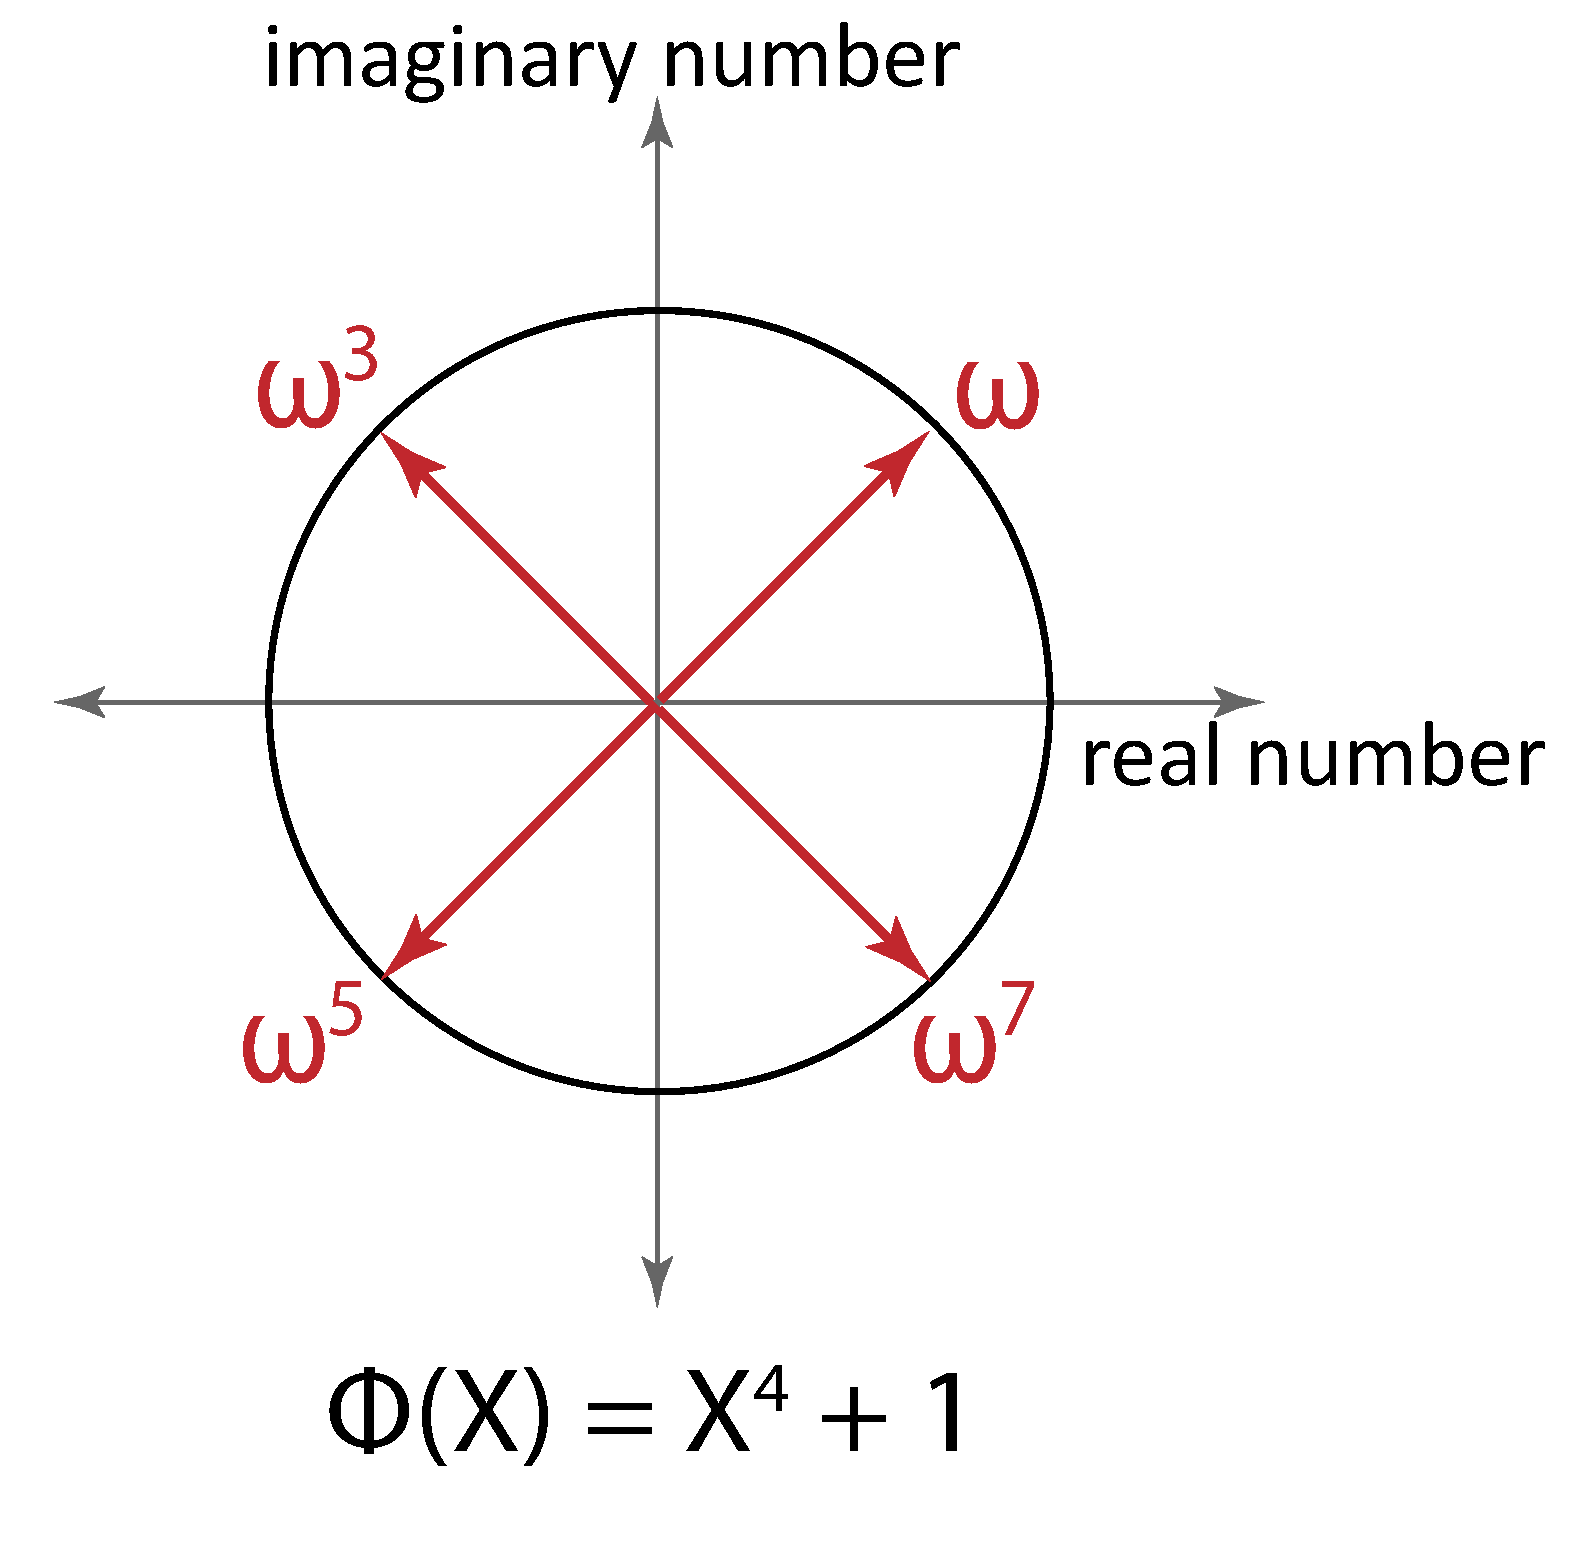
\includegraphics[width=0.3\linewidth]{figures/cyclotomic-polynomial.pdf}
  \caption{An illustration of the four roots of the 8th cyclotomic polynomial $x^4 + 1$ 
  %\href{https://blog.openmined.org/content/images/2020/08/roots.PNG}{(Source)}
  }
  \label{fig:cyclotomic-polynomial}
\end{figure}

$ $

\para{Bijective:} Based on Euler's formula $e^{i\theta} = \cos\theta + i\cdot\sin\theta$ (\autoref{subsec:euler}), we can derive the following arithmetic relations: $\omega = \overline{\omega^{2n-1}}, \text{ } \omega^3 = \overline{\omega^{2n-3}}, \cdots, \omega^{n-1} = \overline{\omega^{n+1}}$. In other words, the one-half roots are conjugates of the other-half roots. This can also be pictorially understood based on a complex plane in \autoref{fig:cyclotomic-polynomial}, where red arrows represent the roots of the 8th cyclotomic polynomial $X^4 + 1$, comprising imaginary number and real number components. As shown in this figure, one half of the red arrows (i.e., roots) are a reflection of the other half on the $x$-axis (i.e., imaginary number axis). This means that we can express these roots as an $n$-dimensional vector whose elements are the roots of $X^n + 1$, such that its second-half elements are a reverse-ordered conjugate of the first-half elements. Based on this vector design, the $\sigma$ mapping can be re-written as follows:

$\sigma(f(X)) = (f(\omega),f(\omega^3),f(\omega^5), \cdots, f(\omega^{n-1}), f(\overline{\omega^{n-1}}), f(\overline{\omega^{n-3}}), \cdots, f(\overline{\omega^3}), f(\overline{\omega}))$

$ $

Since $f(\overline{X}) = \overline{f(X)}$, we can rewrite $\sigma$ as: 

$\sigma(f(X)) = (f(\omega),f(\omega^3),f(\omega^5), \cdots, f(\omega^{n-3}) f(\omega^{n-1}), \overline{f(\omega^{n-1})}, \overline{f(\omega^{n-3})}, \cdots, \overline{f(\omega^3)}, \overline{f(\omega))}$

$ $

This structure of vector exactly aligns with the definition of $\hat{\mathbb{C}}^n$: the first half of the elements of the $n$-dimensional vector $\vec{\hat v}$ is a conjugate of the second half.

For bijectiveness, we also need to demonstrate that every $f(X) \in \mathbb{R}[X] /X^n + 1$ is mapped to some $\vec{\hat v} \in \hat{\mathbb{C}}^{\frac{n}{2}}$, and no two different $f_1(X), f_2(X) \in \mathbb{R}[X] / X^n + 1$ map to the same $\vec{\hat v} \in \hat{\mathbb{C}}^{n}$. The first requirement is satisfied, because each polynomial $f(X) \in \mathbb{R}[X] /X^n + 1$ can be evaluated at the $n$ distinct roots of $X^n + 1$ to a valid number. The second requirement is also satisfied, because in the $(n-1)$-degree polynomial ring, each list of $n$ distinct $(x, y)$ coordinates (where we fix the $X$ values to the $n$ distinct roots of $X^2 + 1$ as $\{\omega, \omega^3, \cdots, \omega^{2n - 1}\}$) can be mapped only to a single polynomial within the $(n-1)$-degree polynomial ring, as proved by Lagrange Polynomial Interpolation (Theorem~\ref*{sec:polynomial-interpolation} in \autoref{sec:polynomial-interpolation}).

$ $

%$\sigma_c$ is bijective, because regardless of whether $X$ is an integer, real or complex number, the a list of $n$ distinct coordinates of $(x, y)$ (where we fix $x$ to be $n$ distinct roots of $X^2 + 1$ over complex numbers) define a unique polynomial within the $(n-1)$-degree polynomial ring. 

\para{Homomorphic:} $\sigma_c$ is homomorphic, because based on the reasoning shown in \autoref{subsec:poly-vector-transformation}, the relations $\sigma(f_a(X) + f_b(X)) = \sigma(f_a(X)) + \sigma(f_b(X))$ and $\sigma(f_a(X) \cdot f_b(X)) = \sigma(f_a(X)) \odot \sigma(f_b(X))$ mathematically hold regardless of whether the type of $X$ is modulo integer or complex number, 

$ $

Since $\sigma_c$ is both bijective and homomorphic over the $(+, \cdot)$ operations, it is isomorphic. 


\begin{tcolorbox}[title={\textbf{\tboxtheorem{\ref*{subsec:poly-vector-transformation-complex}} Isomorphism between Polynomials and Vectors over Complex Numbers}}]

The following mapping $\sigma_c$ between polynomials and vectors over complex numbers is isomorphic:

$\sigma_c: f(X) \in \mathbb{R}[X]/(X^n + 1) \longrightarrow (f(\omega),f(\omega^3),f(\omega^5), \cdots, f(\omega^{2n-1})) \in \mathbb{\hat{C}}^{n} \text{ } (\longrightarrow \mathbb{C}^{\frac{n}{2}})$

$ $

, where $\omega = e^{i\pi/n}$, the root (i.e., the primitive $(\mu=2n)$-th root) of the cyclotomic polynomial $X^n + 1$ over complex numbers, and $\mathbb{\hat{C}}^{n}$ is $n$-dimensional complex special vector space whose second-half elements are reverse-ordered conjugates of the first-half elements. 

\end{tcolorbox}


\subsection{Transforming Basis between Polynomial Ring and Vector Space}
\label{subsec:poly-vector-basis-transfer}


Suppose some polynomials $f_0(X), f_1(X), \cdots, f_{n-1}(X)$ form a basis of the $(n-1)$-degree polynomial ring and $\sigma$ is an isomorphic mapping from the $(n-1)$-degree polynomial ring to the $n$-dimensional vector space $\in \mathbb{Z}^n$. Then, $(\sigma(f_0(X)), \sigma(f_1(X)), \cdots, \sigma(f_{n-1}(X)))$ form a basis of the $n$-dimensional vector space. This is because the $\sigma$-mapped output vectors homomorphically preserve the same algebraic relationships on the $(+, \cdot)$ operations and the basis relationship between basis vectors and a subspace can be expressed as a linear algebraic formula consisting of the $(+, \cdot)$ operations (i.e., linear independence and spanning of the space). Therefore, if a set of polynomials satisfy a basis relationship, their $\sigma$-mapped vectors also preserve a basis relationship.

The same principle holds between a polynomial ring and vector space over complex numbers. Given the polynomial ring $\mathbb{R}[X]/(x^n + 1)$, the most intuitive way to set up a basis of $\mathbb{R}[X]/(x^n + 1)$ is as follows:

$f_0(X) = 1$

$f_1(X) = X$

$f_2(X) = X^2$

$\vdots$

$f_{n-1}(X) = X^{n-1}$

$ $

These $n$ polynomials are linearly independent, because each polynomial exclusively has its own unique exponent term whereas one term cannot be expressed by a linear combination of the other terms. Also, These $n$ polynomials span the polynomial ring $\mathbb{R}[X]/(x^n + 1)$, because each polynomial's scalar multiplication can express any coefficient value of its own exponent term, and summing all such polynomials can express any polynomials in the polynomial ring $\mathbb{R}[X]/(X^n + 1)$.


Now, we will apply the $\sigma_c$ mapping to the above $n$ polynomials that are a basis of the $(n-1)$-degree polynomial ring $\mathbb{R}[X]/(x^n + 1)$. Then, according to the principle of polynomial-to-vector basis transfer (explained in Theorem~\ref*{subsec:polynomial-ring-basis} in \autoref{subsec:polynomial-ring-basis}), we can use these $n$ polynomials (i.e., the basis of the $(n-1)$-degree polynomial ring) and the isomorphic polynomial-to-vector mapping $\sigma_c$ to compute the basis of the $n$-dimensional special vector space $\hat{\mathbb C}^{n}$ as follows: 

$W = \begin{bmatrix}
\sigma_c(f_0(X)) \\
\sigma_c(f_1(X)) \\
\sigma_c(f_2(X)) \\
\vdots \\
\sigma_c(f_{n-1}(X)) \\
\end{bmatrix}
= \begin{bmatrix}
\sigma_c(1) \\
\sigma_c(X) \\
\sigma_c(X^2) \\
\vdots \\
\sigma_c(X^{n-1}) \\
\end{bmatrix}$
$= \begin{bmatrix}
1 & 1 & \cdots & 1 & 1\\
(\omega) & (\omega^3) & (\omega^5) & \cdots & (\omega^{2n-1})\\
(\omega)^2 & (\omega^3)^2 & (\omega^5)^2 & \cdots & (\omega^{2n-1})^2\\
\vdots & \vdots & \vdots & \ddots & \vdots \\
(\omega)^{n-1} & (\omega^3)^{n-1} & (\omega^5)^{n-1} & \cdots & (\omega^{2n-1})^{n-1}\\
\end{bmatrix}$

\text{ } \text{ }  $= \begin{bmatrix}
1 & 1 & 1 & \cdots & 1\\
(\omega) & (\omega^3) & \cdots & (\overline{\omega})^3 & (\overline{\omega})\\
(\omega)^2 & (\omega^3)^2 & \cdots & (\overline{\omega}^3)^2 & (\overline{\omega})^2\\
\vdots & \vdots & \vdots & \ddots & \vdots \\
(\omega)^{n-1} & (\omega^3)^{n-1} & \cdots & (\overline{\omega}^3)^{n-1} & (\overline{\omega})^{n-1}\\
\end{bmatrix}$

$ $

$W$ is a valid basis of the $n$-dimensional special vector space $\hat{\mathbb C}^{n}$. 



\begin{tcolorbox}[title={\textbf{\tboxtheorem{\ref*{subsec:poly-vector-transformation-complex}} Transforming Basis between Polynomial Ring and Vector Space}}]

If $n$ polynomials form a basis of an $(n-1)$-degree polynomial ring and they are converted into $n$ distinct vectors via an isomorphic mapping $\sigma$ (or $\sigma_c$ in the case of the complex number domain) from the $(n-1)$-degree polynomial ring to the $n$-dimensional vector space, then those converted $n$ vectors form a basis of the $n$-dimensional (or $\dfrac{n}{2}$ in the case of the complex number domain) vector space. 

\end{tcolorbox}